%*******10********20********30********40********50********60********70********80

\chap{Background Theory} 
\section{Data science}
It's really important to have a general idea about what "Data Science" means since this thesis procedure is strongly based on the classic Data Science Process.\\
We can define Data Science like a "concept to unify statistics, data analysis and their related methods" in order to understand and analyze actual phenomena with data.\\
It includes theories drawn from many field within the broad areas of mathematics, statistics, information science and computer science.

\begin{figure}[H]
	\centering
    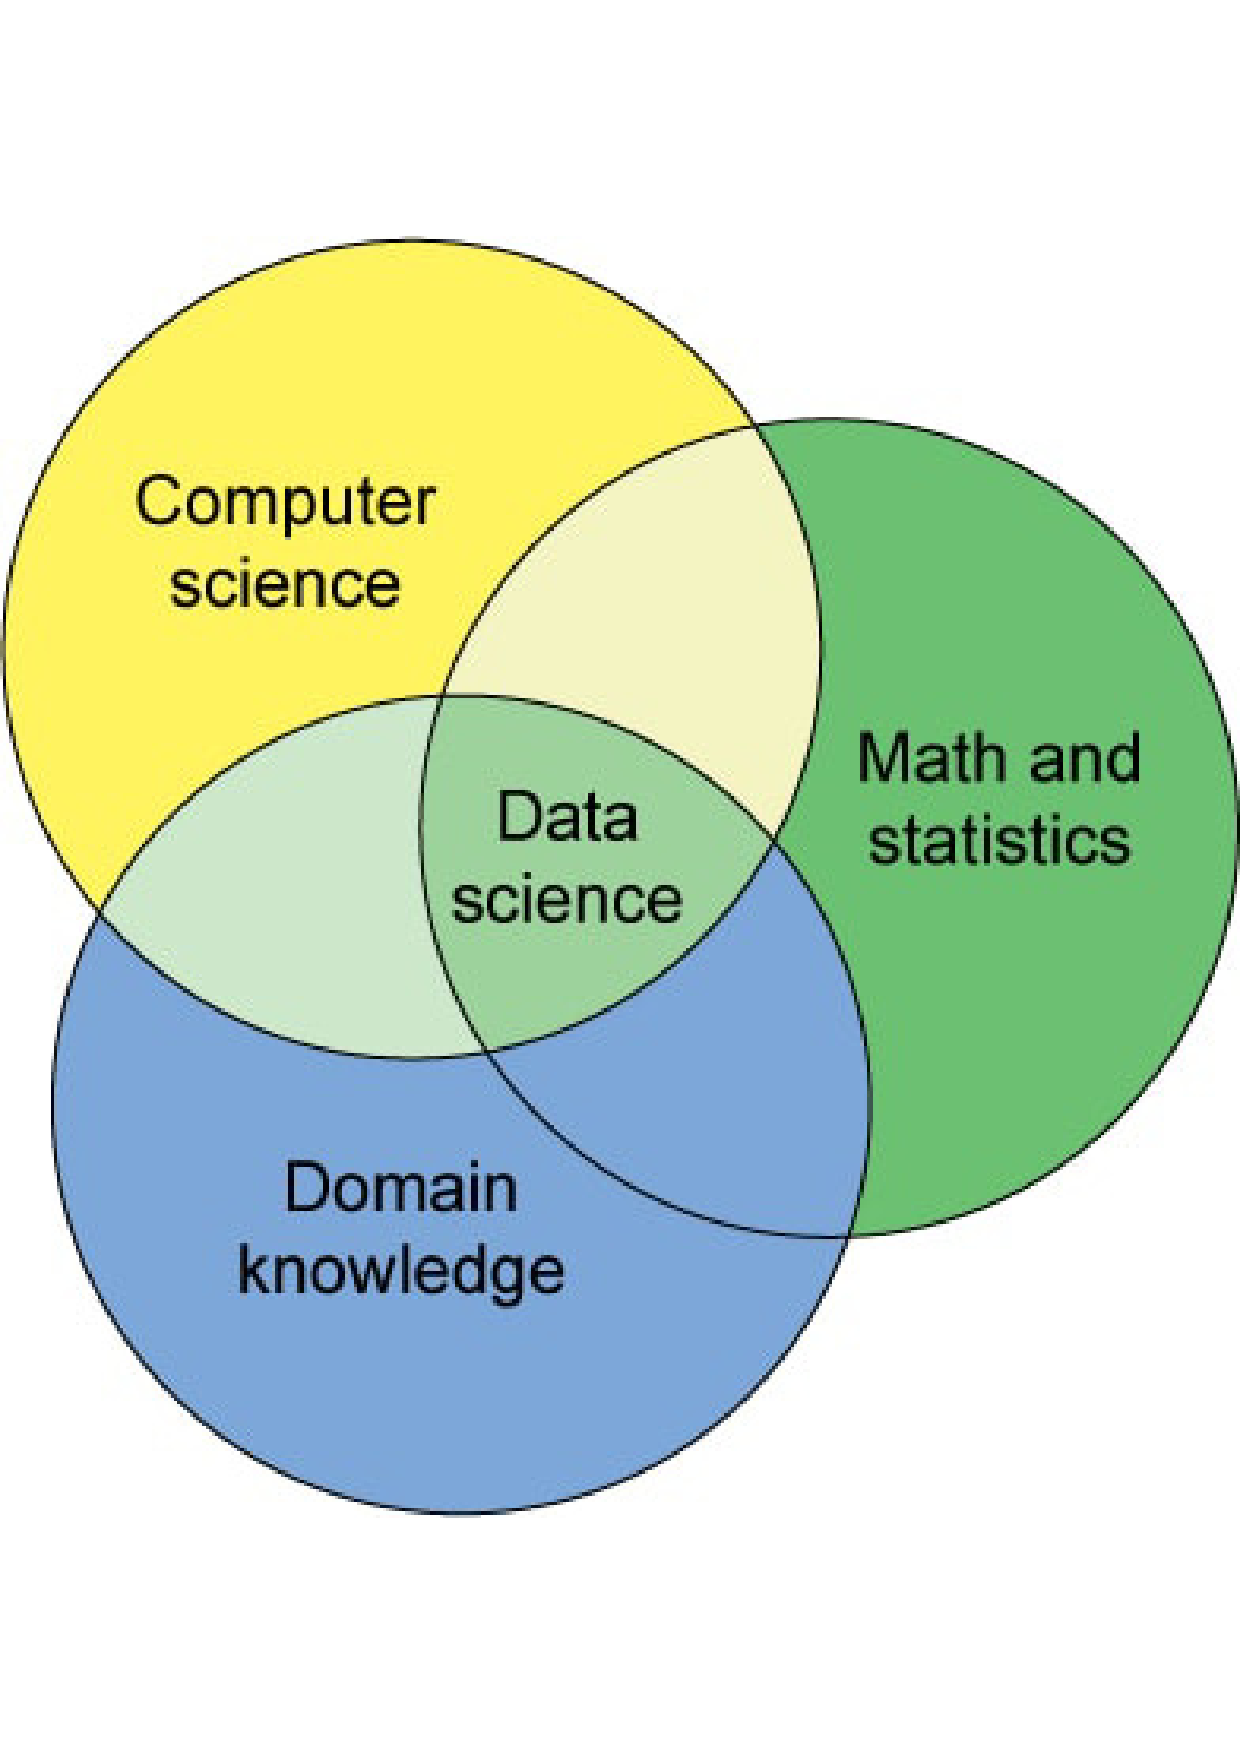
\includegraphics[trim={0 3cm 0 3cm},clip,width=0.4\textwidth]{Files/Data_Science_Concept.pdf}
    \caption{Data science concept}
    \label{fig: Data_science}
\end{figure}

\newpage

In the computer science area are particular important the subdomains of:
\begin{itemize}
\item Machine learning
\item Classification
\item Cluster Analysis
\item Data mining
\item Databases
\item Visualization
\end{itemize}

The follow image represents the "Blitzstein and Pfister's framework" and provides a clear overview of the Data Science process.\\

\begin{figure}[H]
    \centering
    \makebox[\textwidth][c]{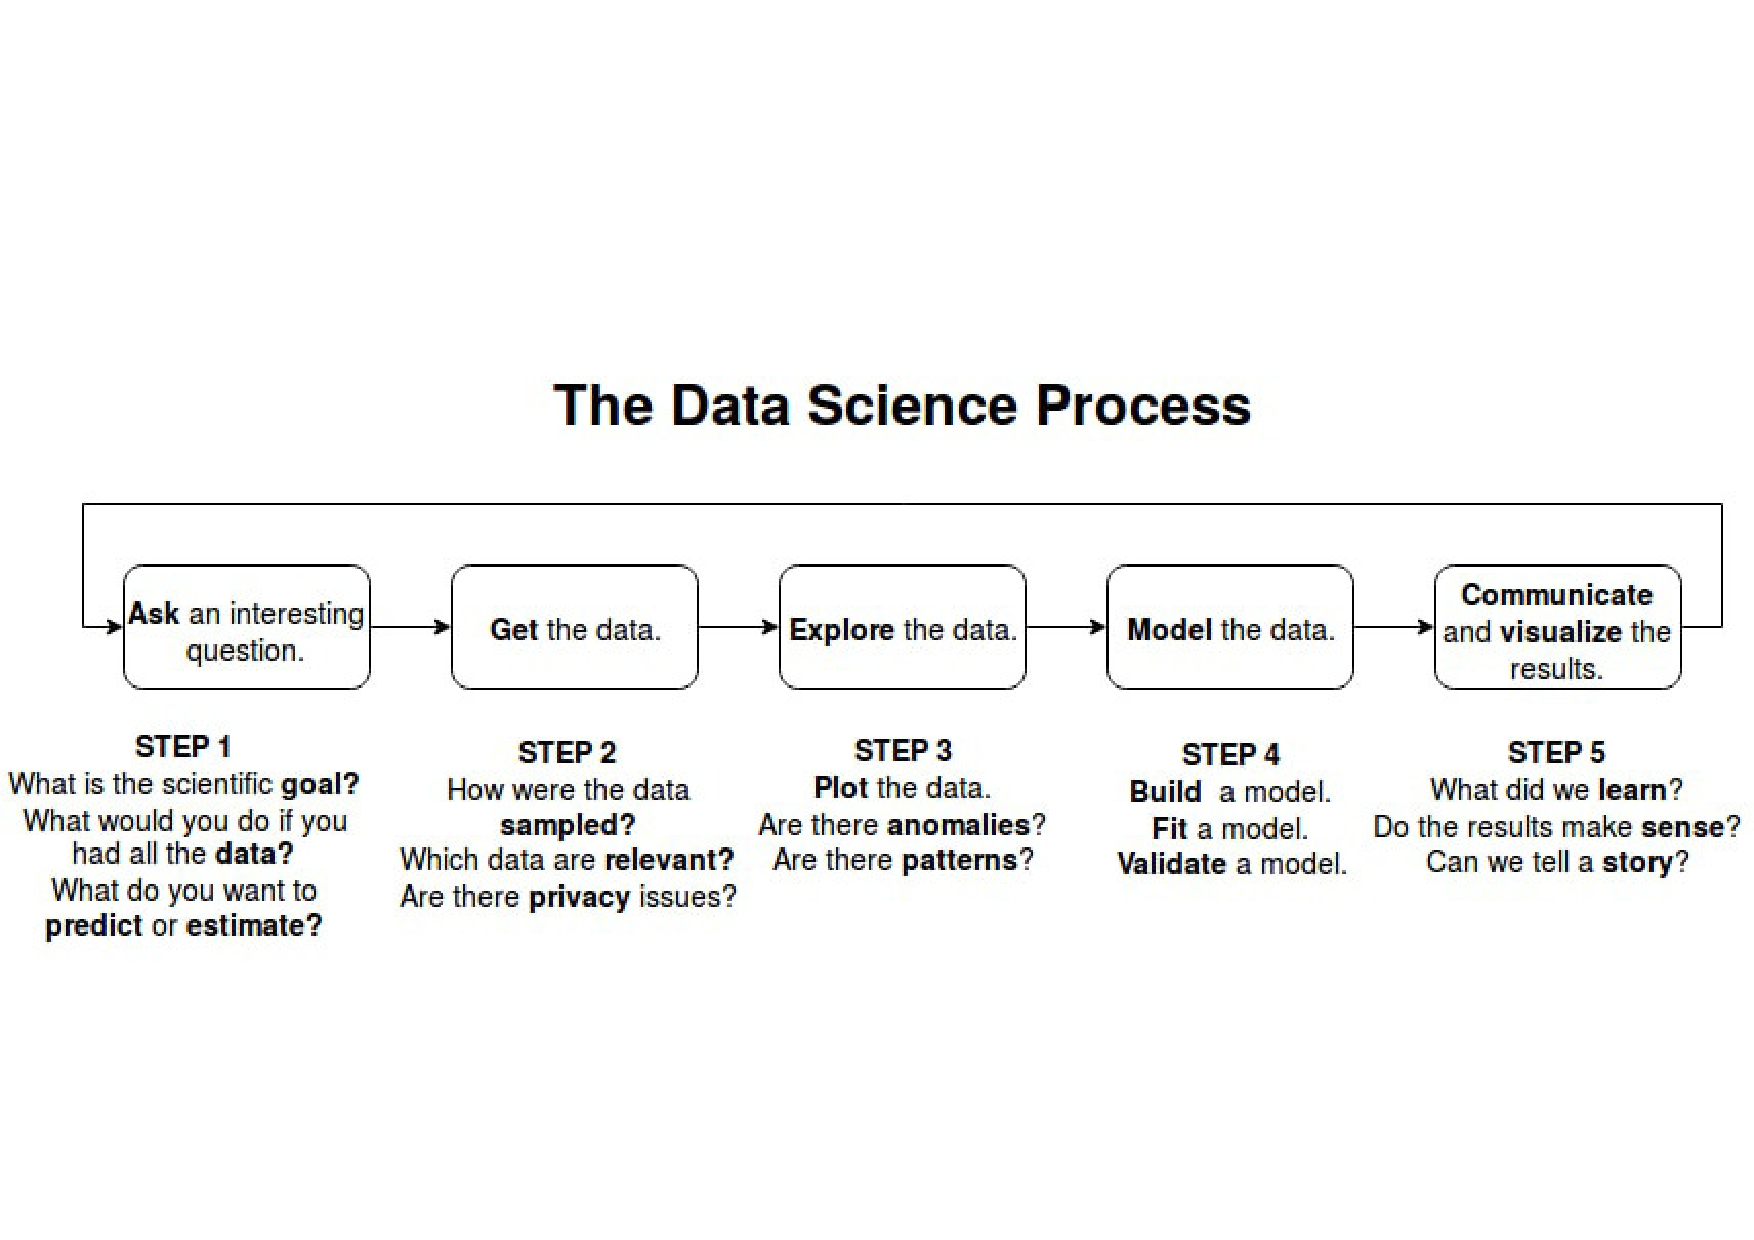
\includegraphics[trim={0 0 0 2cm},clip, width=1.2\textwidth]{Files/Data_Science_Process.pdf}}
    \caption[Data science process]{Data science process}
    \label{fig: Data_science}
\end{figure}



\newpage


\section{Machine learning}
This subfield of computer science gives "computers the ability to learn without being explicitly programmed". \\Evolved from the study of pattern recognition and computational learning theory in artificial intelligence, machine learning explores the study and construction of algorithms that can learn from and make predictions on data.

There are several machine learning algorithm, each one of them is used for a different purpose.The following picture gives a general idea about which categories of algorithms are used and some specific types.


\subsection{Time Series analysis and predictions}
Time Series forecasting is an important area of machine learning, but that is often neglected.

Is that important mainly beause there are so many prediction problems that involve a time component, and these problems are neglected because it is this time component that makes time series problems more difficult to handle.

" A time series is a sequence of observations taken sequentially in time. "
Quoted — Page 1, Time Series Analysis: Forecasting and Control.

Classic example of a time series dataset:\\ 		
Time \#1, observation\\
Time \#2, observation\\
Time \#3, observation

There are different goals depending on wheter we are interested in understanding a dataset or making predictions.

Understanding a dataset is called time series analysis and it can helps to make better prediction, but sometimes it's not required and can result in a large of technocal investment in time and expertise.

Making predictions could be called time series forecasting and it involves taking models fit on historical data and using them to predict future observations.

\subsection{Autoregressive integrated moving average (ARIMA)}

In statistics and econometrics, and in particular in time series analysis, an autoregressive integrated moving average (ARIMA) model is a generalization of an autoregressive moving average (ARMA) model. Both of these models are fitted to time series data either to better understand the data or to predict future points in the series (forecasting).

ARIMA(p, d, q)
\begin{itemize}
\item \textbf{p} is the number of autoregressive terms (How many preceding values are examinated for the current value’s forecast).

\item \textbf{d} is the number of nonseasonal differences needed for stationarity.

\item \textbf{q} is the number of lagged forecast errors in the prediction equation. 
\end{itemize}

\newpage

\section{Aquaculture in Norway}

Is the aquaculture business in Norway growing? 
  
Aquaculture, also known as aquafarming, is the farming of fish, crustaceans, molluscs, aquatic plants, algae, and other aquatic organisms.

Aquaculture would be the future of fish:
In 2030, according to the World Bank, aquaculture will supply:
\begin{itemize}
\item 93.6 Million tonnes of fish per year
\item 25 percent less wild fish will be available
\item 62 percent of the fish we eat will come from farms
\end{itemize}




